\documentclass[xcolor={x11names,table}]{beamer}

\usepackage[overlay,absolute]{textpos}
\setlength{\TPHorizModule}{1cm}
\setlength{\TPVertModule}{1cm}

\usepackage[version=4]{mhchem}

\mode<presentation>
{
\usetheme{default}
\useinnertheme{circles}
\setbeamercovered{transparent}
}

\setbeamertemplate{navigation symbols}{}

\setbeamertemplate{enumerate items}[default]

\setbeamertemplate{footline}{%
	\hfill\scriptsize\textsf{\insertframenumber{}/\inserttotalframenumber}\hspace{0.1cm}\vspace{0.1cm}%
}

\usecolortheme{beaver}
\setbeamercolor{enumerate item}{fg=darkred}
\setbeamercolor{enumerate subitem}{fg=darkred}
\setbeamercolor{enumerate subsubitem}{fg=darkred}
\setbeamercolor{itemize item}{fg=darkred}
\setbeamercolor{itemize subitem}{fg=darkred}
\setbeamercolor{itemize subsubitem}{fg=darkred}
\setbeamercolor{section number projected}{bg=darkred}

\usepackage{graphicx}
\usepackage{url}
\urlstyle{same}

\usepackage[separate-uncertainty=true,detect-none,mode=text]{siunitx}

\usepackage{listings}
%\usepackage{lstlinebgrd}
\lstset{numbersep=4pt, %
	language=Python, % {[ANSI]C}, {[ISO]C++}, {[90]Fortran}, Python, IDL, Java, bash, sh
	numbers=left, % set to none to get rid of line numbers by default
	basicstyle=\ttfamily, % \footnotesize
	%keywordstyle=\color{blue}, %
	%identifierstyle=\color{RoyalBlue4}, %
	commentstyle=\color{Green4}, %
	stringstyle=\color{violet}, %
	showstringspaces=false, % set to true to show spaces visually
	numberstyle=\ttfamily\tiny\color{red}, %
	breaklines=true, %
	tabsize=4 %
}

\usepackage{tikz}
\usetikzlibrary{positioning}
\usetikzlibrary{calc}
\usetikzlibrary{fit}
\tikzstyle{arrow} = [thick,->,>=stealth]

\usepackage{booktabs}

\newcommand{\stabletitle}{PyTorch Crash Course: 0 to MNIST in 1 Hour}

\title{\stabletitle}

\author[markchil] 
{Mark Chilenski\\(markchil)}

\usepackage{ragged2e}

\newcommand{\diff}{\ensuremath{\mathsf{d}}}
\newcommand{\eu}[1][]{\ensuremath{\mathsf{e}^{#1}}}
\newcommand{\pd}[2]{\frac{\partial #1}{\partial #2}}
\newcommand{\TT}{\ensuremath{\mathsf{T}}}

\newcommand{\vect}[1]{\mathbfsf{#1}}
\newcommand{\tens}[1]{\mathbf{#1}}

\DeclareMathOperator{\corr}{corr}
\DeclareMathOperator{\cov}{cov}
\DeclareMathOperator*{\argmax}{arg\,max}
\DeclareMathOperator*{\argmin}{arg\,min}

\newcommand{\todo}[1]{\textcolor{red}{\large\bfseries #1}}

\graphicspath{{../graphics/}}

\AtBeginSection[]
{
  \begin{frame}<beamer>
    \frametitle{\stabletitle}
    \tableofcontents[currentsection]
  \end{frame}
}

\begin{document}

\begin{frame}
 	\titlepage
	
	\begin{center}
		\item You can download the code to follow along at: \url{https://github.com/markchil/pytorch-lecture}
	\end{center}
\end{frame}

\begin{frame}
	\frametitle{Intro}
	About me:
	\begin{itemize}
		\item Graduated 2016 with PhD from Course 22
		\item Currently a research scientist working on a variety of machine learning applications
	\end{itemize}
	Goals for today:
	\begin{itemize}
		\item Cover the core classes/philosophy of PyTorch
		\item Give you enough vocab to confidently google stuff/read the docs
	\end{itemize}
	Prerequisites:
	\begin{itemize}
		\item Basic familiarity with Python
	\end{itemize}
	You can download the code to follow along at: \url{https://github.com/markchil/pytorch-lecture}
\end{frame}

\begin{frame}
	\frametitle{\stabletitle}
	\tableofcontents
\end{frame}

\section{Background: Machine Learning, Neural Networks, and PyTorch}

\begin{frame}
	\frametitle{What Is PyTorch?}
	PyTorch is an open source Python \textbf{machine learning} package geared towards building \textbf{neural networks}, which provides the following key features:\footnote{We'll unpack some of this jargon on the following slides}
	\begin{itemize}
		\item Automatic differentiation
		\item GPU acceleration
		\item Many standard neural network building blocks
		\begin{itemize}
			\item And nice abstractions which make building novel/non-standard ones easy
		\end{itemize}
		\item Rich ecosystem of pre-trained models and open source building blocks
	\end{itemize}
\end{frame}

\begin{frame}
	\frametitle{What Can You Do With PyTorch:\\Machine Learning Crash Course}
	\begin{itemize}
		\item \textbf{Machine learning} refers to algorithms which improve automatically through experience/data
		\item There are various types of machine learning (supervised, unsupervised, reinforcement, etc.)
		\item This crash course focuses on \textbf{supervised learning}:
		\begin{itemize}
			\item The data takes the form of (input, output) pairs
			\item Example: given a picture of a handwritten digit, identify which number was written
		\end{itemize}
	\end{itemize}
	\begin{center}
		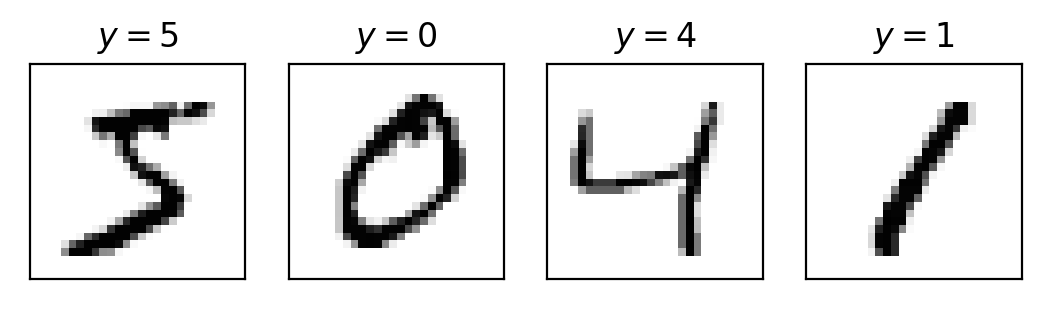
\includegraphics[width=\textwidth]{mnist}
	\end{center}
\end{frame}

\begin{frame}
	\frametitle{PyTorch's Flavor of Machine Learning:\\Neural Network Crash Course}

	\begin{itemize}
		\item PyTorch is geared to a specific family of machine learning approaches: \textbf{(deep) neural networks}
		\item Neural networks are a broad family of models which started out as biologically-inspired data transformations based on networks of ``artificial neurons''
		\begin{itemize}
			\item Modern practice has diverged from these biologically-inspired roots, but some of the terminology remains
		\end{itemize}
	\end{itemize}
\end{frame}

\begin{frame}
	\frametitle{Basic Neural Network Architecture:\\Multi-Layer Perceptron (MLP)}
	Most neural network approaches can be seen as an alternating sequence of linear transformations and (elementwise) non-linear functions:
	\begin{gather*}
		x_{i}=\sigma(W_{i}x_{i-1}+b_{i})
	\end{gather*}
	\begin{itemize}
		\item $\sigma:\mathbb{R}\to\mathbb{R}$ is a nonlinear \textbf{activation function} which is applied separately to each element of its (vector) input
		\item $W_{i}\in\mathbb{R}^{n_{\text{out}}\times n_{\text{in}}}$ and $b_{i}\in\mathbb{R}^{n_{\text{out}}}$ are \textbf{learnable parameters}
	\end{itemize}
	\begin{center}
		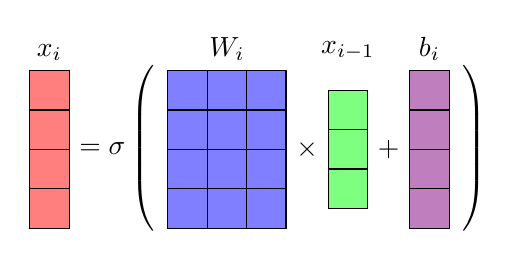
\begin{tikzpicture}
			\node (xout) at (0mm, 0mm) [draw, fill=red, opacity=0.5, minimum width=5mm, minimum height=20mm, anchor=south west] {};
			\foreach \x in {0,...,0}
				\foreach \y in {0,...,3}
					\node at (\x * 5mm, \y * 5mm) [draw, minimum width=5mm, minimum height=5mm, anchor=south west] {};
			\node[right=0mm of xout.east] (phi) {$=\sigma\left(\rule[-10mm]{0pt}{10mm}\right.$};
			\node[right=0mm of phi.east, draw, fill=blue, opacity=0.5, minimum width=15mm, minimum height=20mm, anchor=west] (w) {};
			\foreach \x in {0,...,2}
				\foreach \y in {0,...,3}
					\node [draw, minimum width=5mm, minimum height=5mm, anchor=south west, above right=\y * 5mm and \x * 5mm of w.south west] {};
			\node[right=0mm of w.east] (times) {$\times$};
			\node[right=0mm of times.east, draw, fill=green, opacity=0.5, minimum width=5mm, minimum height=15mm, anchor=west] (xin) {};
			\foreach \x in {0,...,0}
				\foreach \y in {0,...,2}
					\node [draw, minimum width=5mm, minimum height=5mm, anchor=south west, above right=\y * 5mm and \x * 5mm of xin.south west] {};
			\node[right=0mm of xin.east, anchor=west] (plus) {$+$};
			\node [right=0mm of plus.east, anchor=west, draw, fill=violet, opacity=0.5, minimum width=5mm, minimum height=20mm] (b) {};
			\foreach \x in {0,...,0}
				\foreach \y in {0,...,3}
					\node [draw, minimum width=5mm, minimum height=5mm, anchor=south west, above right=\y * 5mm and \x * 5mm of b.south west] {};
			\node [right=0mm of b.east, anchor=west] {$\left. \rule[-10mm]{0pt}{10mm} \right)$};
			\node [above=0mm of xout.north] {$x_{i}$};
			\node [above=0mm of w.north] {$W_{i}$};
			%\node [above=0mm of xin.north] {$x_{i-1}$};
			\path let \p1=(xin.north), \p2=(xout.north) in node [anchor=south] at (\x1,\y2) {$x_{i-1}$};
			\node [above=0mm of b.north] {$b_{i}$};
		\end{tikzpicture}
	\end{center}
\end{frame}

\begin{frame}
	\frametitle{Nuts and Bolts of Neural Network Training:\\Gradient Descent}
	\begin{columns}
		\begin{column}{0.65\textwidth}
			\begin{itemize}
				\item In order to \textbf{train} a neural network with $L$ layers, we need to find values for the parameters $\theta=\{W_{i},b_{i}|1\leq i\leq L\}$
				\item We quantify how good specific parameter values are using a \textbf{loss function} $\mathcal{L}:\Theta\to\mathbb{R}$ which indicates how well the network matches its training data for the given parameters
				\begin{itemize}
					\item Goal is then to find $\hat{\theta}=\argmin_{\theta}\mathcal{L}(\theta)$
					\item Can seek a (local) minimum using \textbf{gradient descent}: update parameters according to
					\begin{gather*}
						\theta_{i+1}=\theta_{i}-\alpha\nabla\mathcal{L}(\theta_{i})
					\end{gather*}
				\end{itemize}
			\end{itemize}
		\end{column}
		\begin{column}{0.45\textwidth}
			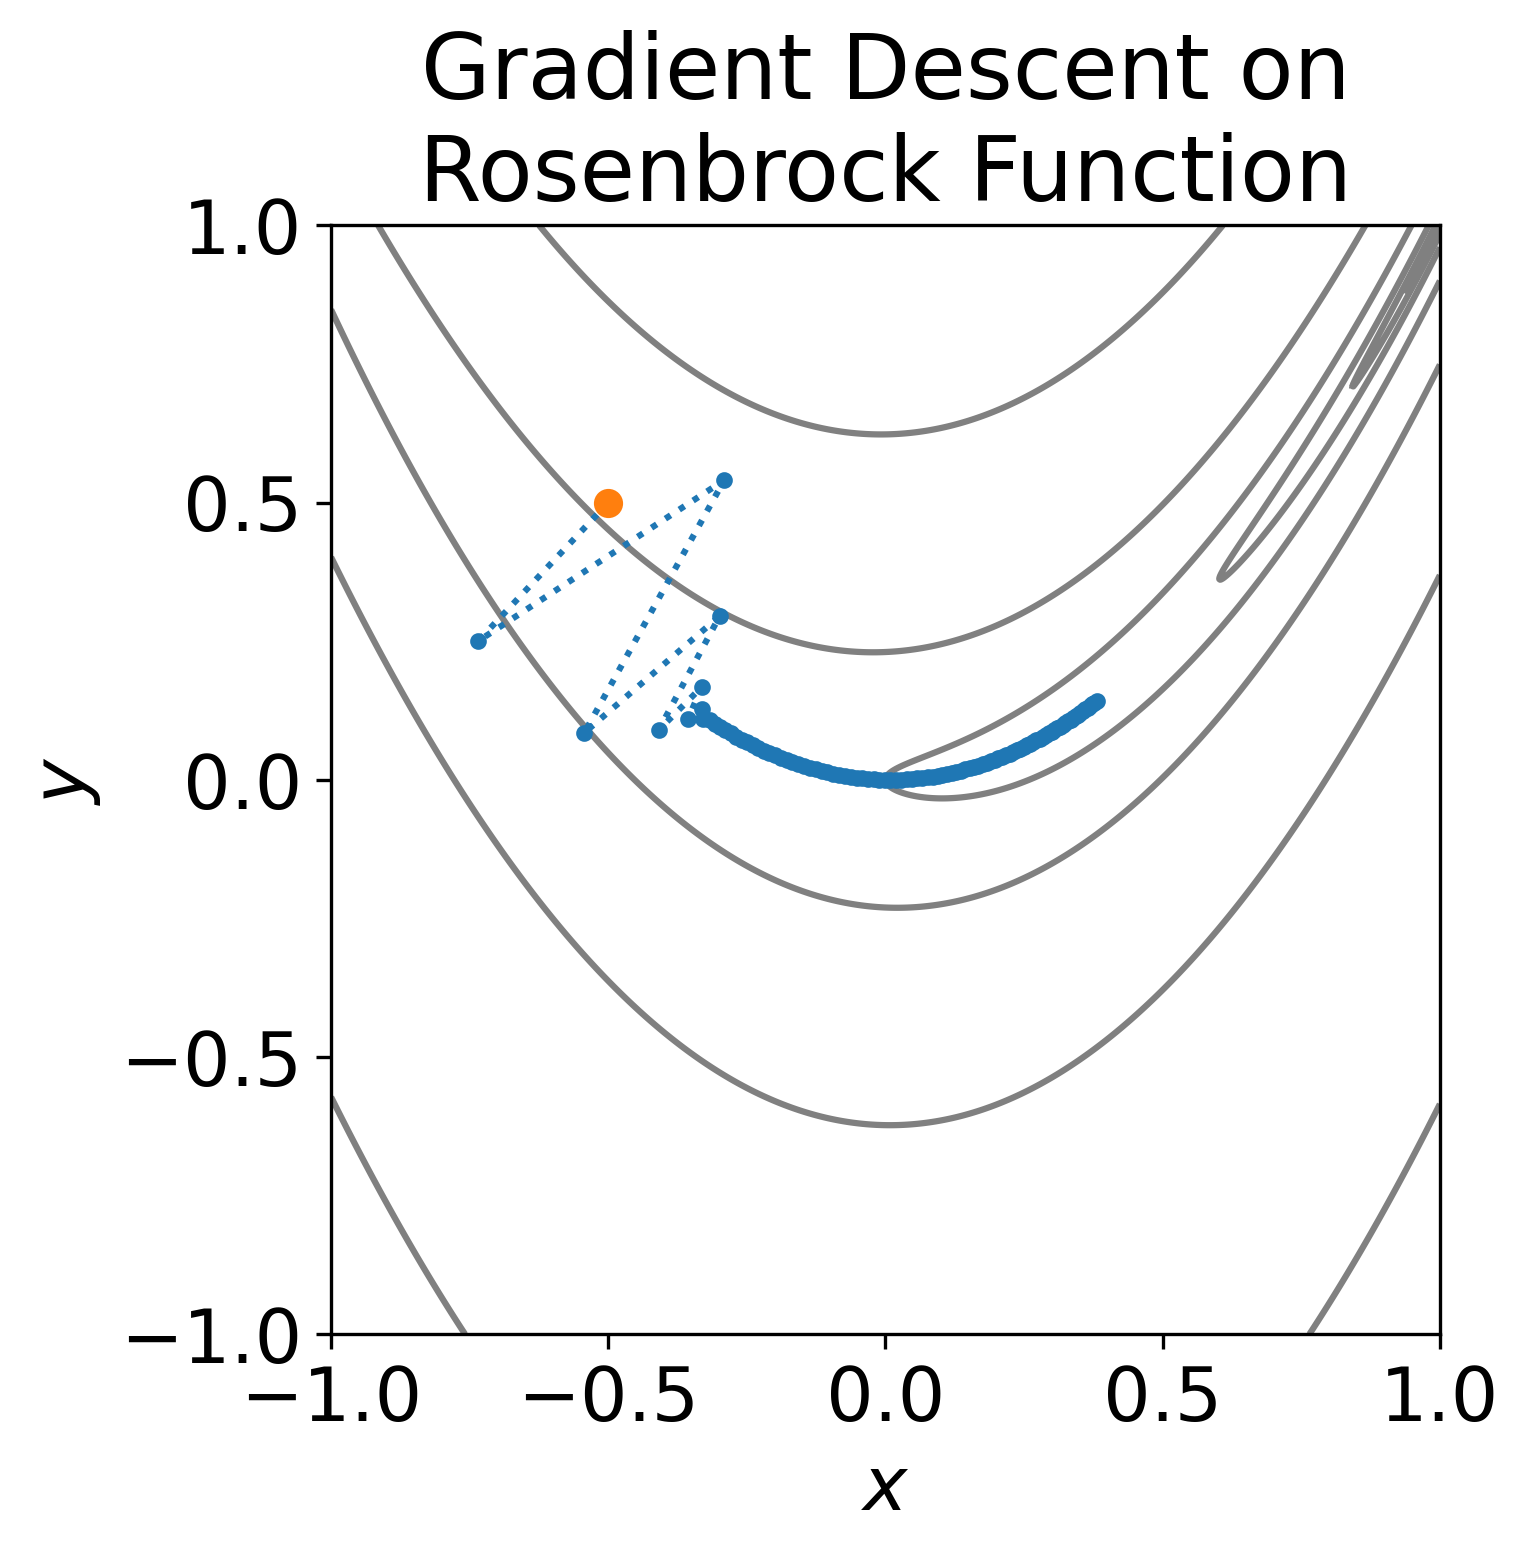
\includegraphics[width=\textwidth]{rosenbrock}
		\end{column}
	\end{columns}
\end{frame}

\begin{frame}
	\frametitle{Why Not Just Write It in NumPy?\\Backpropagation and Automatic Differentiation}
	\begin{itemize}
		\item Gradient descent requires computing the \textbf{gradient} $\nabla\mathcal{L}(\theta_{i})$
		\item The \textbf{backpropagation} algorithm provides an efficient way of doing this, \emph{but needing to write explicit expressions for the gradient of your neural network would be exceedingly tedious and error-prone}
		\item The heart of PyTorch is the ability to perform \textbf{automatic differentiation}: you simply define the loss function computation, and PyTorch automatically computes the gradients for you
	\end{itemize}
\end{frame}

\section{PyTorch Fundamentals: The \lstinline!Tensor! Class}

\begin{frame}
	\frametitle{PyTorch Fundamentals: What Is a Tensor?}
	A tensor $\tens{H}$ of valence $\begin{Bmatrix}\mathfrak{f}\\\mathfrak{v}\end{Bmatrix}$ at a point $\mathfrak{p}$ is a multilinear, real-valued function of $\mathfrak{f}$ 1-forms, and $\mathfrak{v}$ vectors, such that the value of $\tens{H}$ at $\mathfrak{p}$ only depends on the values of the 1-forms and vectors at $\mathfrak{p}$.\footnote{\emph{Visual Differential Geometry and Forms,} T.\ Needham (2021)}
	
	
\begin{tikzpicture}[overlay]
		\only<2>\draw[ultra thick, color=red] (0,0) -- (11,2.25) (11,0) -- (0,2.25);
		\only<2>\node[color=red] at (5.5,0) {\bfseries lol, nope!};
	\end{tikzpicture}
\end{frame}

\begin{frame}
	\frametitle{PyTorch Fundamentals:\\What Does PyTorch Think a Tensor Is?}
	\begin{itemize}
		\item In machine learning, it is common to abuse the word ``tensor'' to refer to any $N$-dimensional array of data
		\item PyTorch's \lstinline!Tensor! class is very similar to the \lstinline!ndarray! class in NumPy, but with some extra machinery attached to:
		\begin{enumerate}
			\item Keep track of gradients
			\item Easily move between CPU and GPU
		\end{enumerate}
	\end{itemize}
\end{frame}

\begin{frame}
	\frametitle{\lstinline!Tensor! Basics}
	A given \lstinline!Tensor! \lstinline!x! consists of several key elements:
	\begin{itemize}
		\item A chunk of memory
		\item A datatype which indicates what type of value is stored in the memory (\lstinline!x.dtype!)
		\item A shape which indicates how the elements are arranged in an $N$-dimensional grid (\lstinline!x.shape!)
	\end{itemize}
\end{frame}

\begin{frame}
	\frametitle{Basics of \lstinline!Tensor! Indexing}
	\begin{itemize}
		\item You can index into a \lstinline!Tensor! just like a Python list, with the added twist that there can be as many indices as there are dimensions:
		\lstinputlisting{../src/indexbasic.py}
		\item There are lots of powerful things you can do by using bool and int \lstinline!Tensors! to index into other \lstinline!Tensors!: the examples here just barely scratch the surface
	\end{itemize}
\end{frame}

\begin{frame}
	\frametitle{Conventional \lstinline!Tensor! Shapes}
	There are a few conventions in use for specific meanings of various dimensions for various types of data:
	\begin{itemize}
		\item Generic data (like for an MLP): shape is (samples, features)
		\item Image data (like for a CNN): shape is (samples, channels, height, width)
		\item Sequence data (like for an RNN):
		\begin{itemize}
			\item Defaults to (steps, samples, features) for RNN/LSTM/GRU
			\item But, I prefer to use the optional (samples, steps, features) form so that the samples dimension is first
		\end{itemize}
	\end{itemize}
\end{frame}

\begin{frame}
	\frametitle{\lstinline!Tensor! Superpowers: Autograd Example}
	\lstinputlisting[firstline=3]{../src/autograd.py}
	
	\begin{itemize}
		\item Symbolically, you would have to find $dz/dx=2x+1$, $dz/dy=1$: \emph{but PyTorch does it automatically for you}
		\item The call to \lstinline!z.backward()! stores $dz/dx$ into \lstinline!x.grad! and $dz/dy$ into \lstinline!y.grad!
	\end{itemize}
\end{frame}


\begin{frame}
	\frametitle{More Details on Autograd}
	\begin{itemize}
		\item Use the \lstinline!requires_grad! keyword to construct a \lstinline!Tensor! which will have gradients computed for it
		\item Use the \lstinline!z.backward()! method to compute gradients of \lstinline!z! with respect to all \lstinline!Tensors! which were involved in its computation
		\begin{itemize}
			\item Gradients of \lstinline!z! with respect to \lstinline!x! are stored in \lstinline!x.grad!
			\item Gradients are \emph{accumulated} with subsequent calls to \lstinline!backward()!: often need to manually zero out gradients
		\end{itemize}
		\item Tracking the computation graph can be expensive: when you do not need gradients, use the \lstinline!no_grad! context manager:
		\lstinputlisting[firstline=3]{../src/nograd.py}
	\end{itemize}
\end{frame}

\begin{frame}
	\frametitle{\lstinline!Tensor! Superpowers: Using a GPU}
	\begin{itemize}
		\item Can easily move \lstinline!Tensors! between GPU and CPU:
		\begin{itemize}
			\item Can create \lstinline!Tensor! on GPU using the \lstinline!device! keyword: \lstinline!x = torch.tensor(1.0, device=torch.device('cuda'))!
			\item Can copy existing \lstinline!Tensor! to GPU using the \lstinline!to()! method: \lstinline!x = x.to(torch.device('cuda'))!
			\item Can copy existing \lstinline!Tensor! to CPU using the \lstinline!cpu()! method: \lstinline!x = x.cpu()!
		\end{itemize}
		\item Best practice: don't hard-code the \lstinline!device! keyword. Instead, make your code fail back to CPU if GPU is unavailable:
		\lstinputlisting[firstline=3]{../src/device.py}
	\end{itemize}
\end{frame}

\section{Higher Abstractions: The \lstinline!torch.nn! Module}

\begin{frame}
	\frametitle{Neural Network Building Blocks: The \lstinline!torch.nn! Module}
	The \lstinline!torch.nn! module has a wide array of standard neural network building blocks, including:
	\begin{itemize}
		\item Linear transformations
		\item Various activation functions
		\item Convolutional layers
		\item Recurrent layers
	\end{itemize}
\end{frame}

\begin{frame}
	\frametitle{Defining an MLP Using \lstinline!torch.nn!}
	\lstinputlisting{../src/sequential.py}
\end{frame}

\begin{frame}
	\frametitle{The \lstinline!Module! Class}
	\begin{itemize}
		\item All of the building blocks in \lstinline!torch.nn! inherit from the \lstinline!torch.nn.Module! class
		\item A given \lstinline!Module! has:
		\begin{itemize}
			\item Parameters: \lstinline!Tensors! which the optimizer should update during training
			\item Buffers: \lstinline!Tensors! which should be included when saving/restoring the \lstinline!Module!, but which should \emph{not} be updated by the optimizer
			\item Submodules: other \lstinline!Modules! which are contained within the \lstinline!Module!
			\item A \lstinline!forward()! method which defines the actual operation performed by the \lstinline!Module!
			\begin{itemize}
				\item Important: never call \lstinline!forward()! directly: \lstinline!Module! provides \lstinline!__call__()! which wraps \lstinline!forward()! with extra steps!
			\end{itemize}
		\end{itemize}
	\end{itemize}
\end{frame}

\begin{frame}
	\frametitle{Some Additional Key \lstinline!Module! Methods}
	\begin{itemize}
		\item \lstinline!to(device)!: Move to the given device
		\begin{itemize}
			\item A \lstinline!Module! and the \lstinline!Tensors! it operates on must be on the same device
		\end{itemize}
		\item \lstinline!train()!: Put into training mode
		\item \lstinline!eval()!: Put into eval mode
		\item \lstinline!parameters()!: Get an iterator over the trainable parameters
	\end{itemize}
\end{frame}

\begin{frame}
	\frametitle{Implementing a Custom \lstinline!Module! Class}
	{
		\small
		\lstinputlisting[firstline=5, lastline=16]{../src/module.py}
	}
\end{frame}

\begin{frame}
	\frametitle{Using the Custom \lstinline!Module!}
	\lstinputlisting[firstline=19]{../src/module.py}
\end{frame}

\begin{frame}
	\frametitle{Saving/Loading \lstinline!Modules!}
	\begin{itemize}
		\item The \lstinline!state_dict()! method returns a dict which has the values of all of the parameters and buffers associated with a given \lstinline!Module!
		\item This can be saved to disk, and restored using the \lstinline!load_state_dict()! method
	\end{itemize}
	\lstinputlisting[firstline=4]{../src/saverestore.py}
\end{frame}

\section{Data Handling: The \lstinline!Dataset! and \lstinline!DataLoader! Classes}

\begin{frame}
	\frametitle{Two-Stage Data Handling: \lstinline!Dataset! and \lstinline!DataLoader!}
	PyTorch breaks down data handling into two steps:
	\begin{enumerate}
		\item A \lstinline!Dataset! provides a wrapper to access single (input, output) pairs at a time
		\item A \lstinline!DataLoader! combines multiple samples from a \lstinline!Dataset! into batches
	\end{enumerate}
	Both of these classes are defined in \lstinline!torch.utils.data!
\end{frame}

\begin{frame}
	\frametitle{\lstinline!Dataset!: Single-Sample Access}
	To get your data into PyTorch's format, you simply need to subclass \lstinline!Dataset! and implement two methods:
	\begin{itemize}
		\item \lstinline!__len__()!: returns the number of samples in the \lstinline!Dataset!
		\begin{itemize}
			\item It is usually safe to change the length over time: a \lstinline!Dataset! can grow/shrink
		\end{itemize}
		\item \lstinline!__getitem__(idx)!: returns the sample at a given index
		\begin{itemize}
			\item Can do arbitrary processing here: e.g., load image from disk, crop, scale, convert to \lstinline!Tensor!, etc.
			\item Can return fairly arbitrary output, as long as the result at each index has the same form
			\item Do not always need to return the same value for a given index: a \lstinline!Dataset! can perform random data augmentations or even data generation
		\end{itemize}
	\end{itemize}
\end{frame}

\begin{frame}
	\frametitle{\lstinline!TensorDataset! Example}
	If your data are already stored in \lstinline!Tensors!, can simply wrap them with a \lstinline!TensorDataset!:
	\lstinputlisting[firstline=4]{../src/tensordataset.py}
\end{frame}

\begin{frame}
	\frametitle{\lstinline!DataLoader!: Sampling and Batching}
	\begin{itemize}
		\item Typically train using \textbf{mini-batch stochastic gradient descent}: update the trainable parameters using gradients computed from a random subset of the training data
		\item \lstinline!DataLoader! wraps a \lstinline!Dataset! and enables iteration over batches
	\end{itemize}
	{
		\small
		\lstinputlisting[firstline=4]{../src/dataloader.py}
	}
\end{frame}

\section{Putting It All Together to Solve MNIST: The ``\texttt{hello, world}'' of Machine Learning}

\begin{frame}
	\frametitle{MNIST: The ``\texttt{hello, world}'' of Machine Learning}
	\begin{itemize}
		\item One of the standard image processing benchmark datasets for many years
		\item Consists of $28\times 28$ grayscale images of handwritten digits: \num{60000} training images and \num{10000} test images
		\begin{itemize}
			\item Data are very clean: only one digit per image, nicely centered/scaled, etc.
		\end{itemize}
		\item Fairly small/easy by today's standards, but good for education because you can successfully train models on the CPU
	\end{itemize}
	\begin{center}
		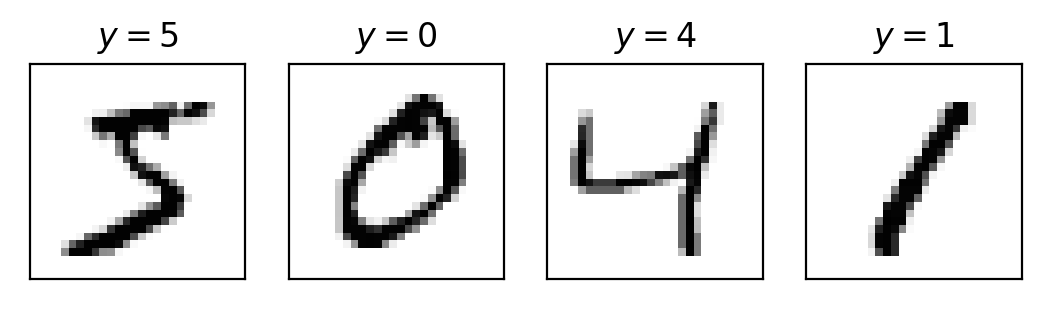
\includegraphics[width=\textwidth]{mnist}
	\end{center}
\end{frame}

\begin{frame}
	\frametitle{Solution Script (Walk Through Full Code in Editor)}
	\vspace{-0.5\baselineskip}
	{
		\scriptsize
		\lstinputlisting[firstline=45]{../src/mnist/mnist.py}
	}
\end{frame}

\begin{frame}
	\frametitle{Example Output (Last Few Lines)}
	\lstinputlisting[firstline=31]{../src/mnist/output.txt}
\end{frame}

\section{Summary and Resources}

\begin{frame}
	\frametitle{Summary and Additional Resources}
	PyTorch-specific resources:
	\begin{itemize}
		\item PyTorch documentation: \url{https://pytorch.org/docs/stable/index.html}
		\item PyTorch tutorials: \url{https://pytorch.org/tutorials/}
		\item PyTorch book: \url{https://pytorch.org/assets/deep-learning/Deep-Learning-with-PyTorch.pdf}
	\end{itemize}
	
	General machine learning/deep learning resources:
	\begin{itemize}
		\item Introduction to Statistical Learning (R-focused, but very popular for learning the fundamentals): \url{https://www.statlearning.com/}
		\item Probabilistic Machine Learning (book series): \url{https://probml.github.io/pml-book/}
		\item Deep Learning: \url{https://www.deeplearningbook.org/}
	\end{itemize}
\end{frame}

\end{document}